\section{Background}
%\frame{
%	\frametitle{Treatment Options}
%	
%	\begin{center}
%		\includegraphics[width=0.88\textwidth]{../../IROS2017/Google/figures/treatment.jpg}
%	\end{center}
%	
%	\begin{itemize}
%		\item Radiotherapy treatment is the most effective
%	\end{itemize}
%} 

\begin{frame}
	\frametitle{Three Dimensional Conformal Radiation Therapy}
	%
	\begin{itemize}
		\tiny \item Intensity Modulation: Control external beam's physical delivery
		\tiny \item \textit{Conform} internally uniform fields with MLCs using a projection of target volumes [~\cite{boyer1992clinical}]
		\tiny \item Improve tumor's local control
	\end{itemize}
%
	\begin{columns}[c]
		\begin{column}{.55\textwidth}	
			\centering		
			\includegraphics[width=.55\linewidth, rotate=90]{../../../Proposal/figures/cfrt_imrt.png}\\			
			%
			\tiny L-R: Conventional radiotherapy. Conformal radiotherapy (CFRT) without intensity modulation.  CFRT with intensity modulation. Reprinted from~\cite{WebbIMRT}.
		\end{column}
	%	
	\begin{column}{.48\textwidth}
		\includegraphics[width=.92\linewidth]{../../../PhDThesis/figures/varian_mlc.jpg} \\
		\centering \tiny{A multi-leaf collimator for IMRT/3DCRT. \copyright Varian Medical Systems.}
		\label{fig:mlc_varian}
	\end{column}
	\end{columns}
\end{frame}


\subsection{Conformal RT Treatment Planning Parameters}
\frame{
	\frametitle{Conformal RT Treatment Planning Parameters}
	\begin{itemize}
		\item Optimal treatment \textit{parameters} $\rhd$ good treatment outcome
		%
		\vspace{0.05in}
		%
		\begin{itemize}
			\item dose-limiting structures
			%
			\vspace{0.1in}
			%
			\item OARs within a {target volume}
			%
			\vspace{0.1in}
			%
			\item doctor's {dose prescription}
			%
			\vspace{0.1in}
			%
			\item {dose fractionation}
			%
			\vspace{0.1in}
			%
			\item  \textbf{patient positioning}
			%
			\vspace{0.1in}
			%
			\item \textbf{dose distribution}
		\end{itemize}
	\end{itemize}
}

\subsection{Robot-based Radiation Therapy}
\frame{
	\frametitle{Frame-based Radiotherapy Treatment}
	\begin{itemize}
		\tiny \item Accurately irradiate a \textit{moving target} and a \textit{moving patient} with the aid of robots[\cite{Schweikard95, Webb99Robotic}]
%		\item Head landmarks and rigid mechanical immobilization mechanisms
		\begin{columns}[c]
			\begin{column}{.89\textwidth}
				\includegraphics[width=0.5\linewidth]{../../IROS2017/Google/figures/frame1.jpg}
				\-
				\hspace{0.25em}
				\includegraphics[width=0.450\linewidth]{../../IROS2017/Google/figures/frame2.jpg}
			\end{column}
		\end{columns}
	\end{itemize}	
}

\subsection{Frameless and Maskless: Cyberknife system}
\begin{frame}
\frametitle{Frameless and Maskless Radiotherapy}
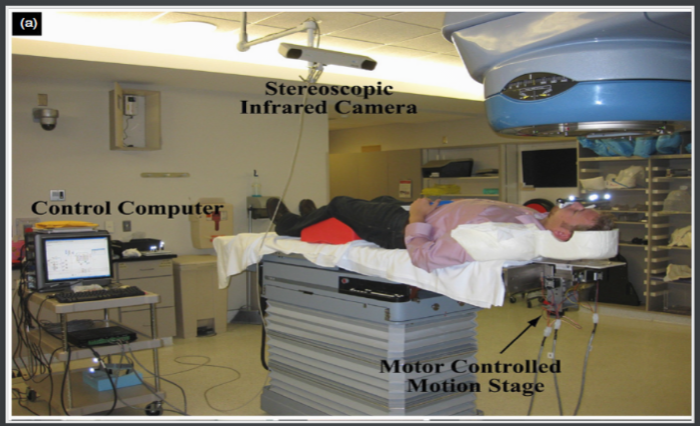
\includegraphics[width=\columnwidth]{figures/igrt.png}
\centering \copyright ~\cite{Wiersma09Dev}
\end{frame}

\begin{frame}
\frametitle{HexaPOD}
\centering 
\includegraphics[width=\columnwidth]{../../../PhDThesis/figures/hexapod.png} \\
\centering Reprinted from \cite{HerrmannHexaPODMPC}
\end{frame}

\begin{frame}
\frametitle{Cyberknife/Novalis systems}
\begin{columns}[c]
	\begin{column}{0.5\textwidth}
		\centering				
		\includegraphics[width=\linewidth]{../../../BOO/figures/cyberknife.jpg}
	\end{column}
	%
	\begin{column}{0.5\textwidth}
		\centering				
		\includegraphics[width=\linewidth]{../../../BOO/figures/cyberknife_rotating.jpg}
%		\includegraphics[width=\linewidth]{../../../Proposal/figures/novalis.png}
	\end{column}
\end{columns}
\end{frame}
%
\begin{frame}
\frametitle{The Novalis ExacTrac Module}
\centering %The Novalis ExacTrac Module
\includegraphics[width=\columnwidth]{../../../Proposal/figures/novalis.png}
\centering \copyright Novalis
\end{frame}

\frame{
	\frametitle{The Case for Soft Robots}
	\begin{itemize}
		\item Frame-based immobilization 
		%
		\vspace{0.1in}
		%
		\begin{itemize}
			\item LINAC misalignments $\implies$ negative dosimetry effects %[\cite{soft_robot:c2}]
			%
			\vspace{0.1in}
			%
			\item $\times$ Fractionated treatments
			%
			\vspace{0.1in}
			%
		\end{itemize}
		\item Frameless RT
		\begin{itemize}
			\item Incompatible with most conventional LINACs 
		\end{itemize}
		%
		\vspace{0.1in}
		%
		\item Cyberknife/Novalis Systems
		%
		\vspace{0.1in}
		%
		\begin{itemize}
			\item Reliance on pre-treatment images
			%
			\vspace{0.1in}
			%
			\item Rigid motion compensation issues
		\end{itemize}
	\item Involuntary patient motion requires adaptive positioning 
	\end{itemize}
\footnotetext{\tiny Morphological computation, Cephalopods, Adaptive Controller for changing head dynamics: shape, weight etc}
}

\subsection{BOO}
\begin{frame}
	\frametitle{Beam Orientation Optimization}
	\begin{itemize}
		\item During treatment planning, a \textbf{b}eam \textbf{o}rientation \textbf{o}ptimization problem (BOO) is  separately solved
		%
		\vspace{0.1in}
		%
		\item Radiation is delivered from
		$\approx(5 − 15)$ different beam orientations during IMRT
		%
		\vspace{0.1in}
		%
		\item BOO determines the best beam angle combinations for delivering radiation
		%
		\vspace{0.1in}
		%
		\item Process of determining beamlets' intensities is termed \textbf{fluence map optimization} (FMO)
	\end{itemize}
\end{frame}